\section{Simulation Results}
%\begin{itemize}
%    \item Simulation Results
%    \item Fullscale test Results
%    \item Discussion som tar for seg både simulator of fullskalatest i ett delkapittel.
%    \item ALTERNATIVT: Et kapittel for simulator, et kapittel for fullskalatest, Diskusjon som eget kapittel etter begge som samler og diskuterer all resultatene.
%\end{itemize}

\iffalse
\begin{itemize}
    \item noen større scenarioer, noen enkle situasjoner. For å vise hvordan algoritmen oppfører seg i forskjellige situasjoner med varierende kompleksitet.
    \item Delkapittel for hver "stor" scenario, et delkapittel for alle 'enkle' situasjoner.
    \item Viktig å analysere både bra, dårlig, og uvented oppførsel.
    \item annen viktig sak som må diskuteres er hvor 'inconsistent' oppførselen er, små endringer i scenario innstillinger gir store utslag på oppførselen vår.
    \item Se på forskjell i oppførsel mellom når vi har 'prediksjon' av target ships og når vi bare antar fast kurs og hastighet.
\end{itemize}
\fi

To test the capabilities of the trjectory planning algorithm it is useful to conduct simulations of vareous scenarios.
With a simulator it is possible to cover a wide assortment of scenarios in a timely fashion, this helps explore the full
range of the algorithm's behaviour without having to conduct time consuming full scale tests. NTNU also has a full-scale
functional prototype of an autonomous ferry that could be used to conduct real life tests. However during the period of working
on this thesis the ferry was out of commission due to a thruster failure.
The MATLAB simulator emlpoyed for this thesis was developed by Emil Thyri and is used with permission. In this chapter the results
are presented with figures to show the developemnt of the scenario over time, in addition to these figures there exists a youtube video compiling
all the results in video format, the video can be found as an attachment to the thesis, or by following this link: (TODO: sett in link).

All the simulations are conducted under the assumption that the \gls{OS} has perfect vision for spotting and tracking dynamic obstacles.
disturbances are also largely ignored, the simulation features no current or wind induced sideslip, crab angle is also not considered.

\subsection{scenario overview}
\iffalse
Flere ting å teste:
Scenario der det er en statisk hindring midt i referanse banen.
Scenario der vi mer tydelig blir 'dyttet' inn mot statisk hindring av annen båt.
Scenario der det er overlap mellom forskjellige COLREGs situasjoner
Scenario med flere båter i samme COLREGs situasion, kan kombineres med scenario over.
Skjaergård MÅ inkludere en bane gjennom masse små skjær, ikke fordi det er vanlig men fordi det må testes.

\begin{itemize}
    \item Havn
    \subitem crossings, head-on, trangt med statiske hindringer, full blockade av veien vi skal ta.
    \subitem kan variere stat posisjoner for å se endra flere forskjellige COLREGs situasjoner.
    \item 'Trondheimsfjord'
    \subitem Større åpent hav, mange båter på kryss og tvers.
    \subitem viser at båter som vi vet vi ikke kommer i nærheten av ikke påvirker oppførselen vår.
    \subitem viser at vi kan tracke en referanse veldig godt.
    \item 'Skjærgård'
    \subitem Litt i samme stil som 'Trondheimsfjord', men flere små statiske hindringer.
    \subitem viser fint hvordan små statiske hindringer fortsatt blir 'oppdaget'.
    \subitem stor distanse $\rightarrow$ lang tidshorisont og hvordan det påvirker oppførselen vår.
    \item 'usynlig sving'
    \subitem Traffikert område hvor 'all' trafikken følger en spesifikk sving.
    \item enkle situasjoner:
    \subitem Head-on, Give way, Stand on i 'åpent' hav med bare et target ship.
    \subitem med og uten sving inkludert, for prediksjons sammenligning.
\end{itemize}

\fi

The scnearios used for this thesis are constructed to test both trajectory planning and collision avoidance capabilities through
a combination of both trivial and complex situations. The scenarios are also designed so that behaviour differences between
full and simple \gls{Ts} prediction can be observed. Any time we encounter a \gls{Ts} that maintains a steady course and
velocity there will not be any observable difference, therefor most of the scenarios are constructed so that encounters occur
when ships are turning.
The first set of scenarios are simple situations to establish baseline behaviour in the vareous \gls{COLREGs} situations. In these scenarios there are only 
two agents and there are mostly no meaningful differences observed between simle and full prediction of \gls{Ts}s. 
The second set of scenarios are more complex by featuring more agents and longer paths to follow. These scenarios often feature multiple \gls{COLREGs} situations that can
even overlap, additionally \gls{Ts}s will not be considerate of the \gls{OS} and will exhibit reckless behaviour in order to test a sort of worst case scenario.
The complex scenarios also incorporate static obstacles. (TODO: Her må det skrives litt mer om hvordan og hvorfor osv.)


\subsubsection*{Simple COLREGs situations}
These scenarios feature two agents, the \gls{OS} and the \gls{Ts}, each entering a fully open space while maintaining a
steady course and fixed speed. The agents then cross in manners as described by the \gls{COLREGs} rules discussed in prior chapters.


\subsubsection*{Turning COLREGs situations}
Similar to the simple \gls{COLREGs} situations these scenarios all feature two agents who enter a fully open space. The difference
is as the name implies that these scenarios feature a turn by the \gls{Ts}. Shortly after both agents are in motion the \gls{Ts}
will alter it's course, changing the COLREGs situation from one apparent situation to another.

\subsubsection*{Canals}
This scenario features a set of canals that form a T-junction as well as a choke point on one of the junction points that restricts
the traversable space. There are three agents present and they all meet roughly at the choke point, the scenario is set up so that
the dynamic constraints of the \gls{Ts}s completely block the path of the \gls{OS} if full prediction is used.

\subsubsection*{Helloya}
The situation in this scenario is specifically modelled after a spot Brønnøysund and is not an entirely uncommon
situation when in transit along the coast of Norway. Traffic that wishes to avoid the narrow pass leading in to or out of
Brønnøysund's will elect to take a wider path on the outside of the local archapeligo. The result is a path with a very prominent
turn that is invisible at a glance, but very obvious to any experienced navigator. The simulation is conducted with the \gls{OS} arriving
from both the north and south direction with both full and simple prediction enabled. 

\subsubsection*{Skjærgård}
(TODO: har lyst å endre plassering av statiske hindringer for dette scenarioet, og kanskje scrumpe inn distansen litt.
Det er allerede bevist at algoritmen klarer å følge en bane som tar mer enn 5 minutter å reise gjennom.)

\subsubsection*{Trondheimsjord}
(TODO: Har lyst å endre denne så det er mange flere aktive situasjoner som baller seg på, dette blir da en slags stresstest av
COLREGs compliance, selv om det også blir ett veldig urealistisk worst case scenario der ingen av target ships bryr sæg særlig om reglene.)

\subsubsection*{miscellaneous}
These scenarios are not meant to simulate any specific situation, rather these are meant to showcase quirks, features, and bugs
encountered while developing and testing the algorithm. While some of the problems shown here were taken care of and are no longer present in the
current iteration of the algorithm they are nonetheless important to showcase and discuss.


\subsection{Results}
\begin{itemize}
    \item 'Dårlig' resultat er fortsatt resultat
\end{itemize}



\subsubsection{Simple Head On}
\begin{figure}[!b] %TODO: Skriv. Enkel HO sim med og uten constraints
    \begin{subfigure}[b]{0.49\textwidth}
        \centering
        \includegraphics[width=\textwidth]{Images/Figures/Enkel_HO/Simple0_f1_Frame1}
        \subcaption{caption}
    \end{subfigure}
    \hfill
    \begin{subfigure}[b]{0.499\textwidth}
        \centering
        \includegraphics[width=\textwidth]{Images/Figures/Enkel_HO/Simple0_f600_Frame1}
        \subcaption{mhm}
    \end{subfigure}
    \hfill
    \\
    \begin{subfigure}[b]{0.49\textwidth}
        \centering
        \includegraphics[width=\textwidth]{Images/Figures/Enkel_HO/Simple0_f1_Frame2}
        \subcaption{caption}
    \end{subfigure}
    \hfill
    \begin{subfigure}[b]{0.499\textwidth}
        \centering
        \includegraphics[width=\textwidth]{Images/Figures/Enkel_HO/Simple0_f600_Frame2}
        \subcaption{mhm}
    \end{subfigure}
    \hfill
    \\
    \begin{subfigure}[b]{0.49\textwidth}
        \centering
        \includegraphics[width=\textwidth]{Images/Figures/Enkel_HO/Simple0_f1_Frame3}
        \subcaption{caption}
    \end{subfigure}
    \hfill
    \begin{subfigure}[b]{0.499\textwidth}
        \centering
        \includegraphics[width=\textwidth]{Images/Figures/Enkel_HO/Simple0_f600_Frame3}
        \subcaption{mhm}
    \end{subfigure}
    \hfill
    \caption{TODO: Skriv. Enkel HO sim med og uten constraints}
\end{figure}% 

\begin{figure}[!b]%TODO: Enkel HO w\_opt
    \centering 
    \begin{subfigure}[b]{0.61\textwidth}
        \centering
        \includegraphics[width=\textwidth]{Images/Figures/Enkel_HO/Simple0_f999_Frame1}
        \subcaption{TODO: Skriv}
    \end{subfigure}
    \hfill 
    \begin{subfigure}[b]{0.61\textwidth}
        \centering
        \includegraphics[width=\textwidth]{Images/Figures/Enkel_HO/Simple0_f999_Frame2}
        \subcaption{TODO: Skriv.}
    \end{subfigure}
    \hfill
    \begin{subfigure}[b]{0.61\textwidth}
        \centering
        \includegraphics[width=\textwidth]{Images/Figures/Enkel_HO/Simple0_f999_Frame3}
        \subcaption{TODO: Skriv.}
    \end{subfigure}
    \caption{TODO: Enkel HO w\_opt}
\end{figure}

\subsubsection{Simple Give Way}
\clearpage
\begin{figure}[!b] %TODO: Skriv. Enkel GW sim med og uten constraints
    \begin{subfigure}[b]{0.49\textwidth}
        \centering
        \includegraphics[width=\textwidth]{Images/Figures/Enkel_GW/Simple0_f1_Frame1}
        \subcaption{caption}
    \end{subfigure}
    \hfill
    \begin{subfigure}[b]{0.499\textwidth}
        \centering
        \includegraphics[width=\textwidth]{Images/Figures/Enkel_GW/Simple0_f600_Frame1}
        \subcaption{mhm}
    \end{subfigure}
    \hfill
    \\
    \begin{subfigure}[b]{0.49\textwidth}
        \centering
        \includegraphics[width=\textwidth]{Images/Figures/Enkel_GW/Simple0_f1_Frame2}
        \subcaption{caption}
    \end{subfigure}
    \hfill
    \begin{subfigure}[b]{0.499\textwidth}
        \centering
        \includegraphics[width=\textwidth]{Images/Figures/Enkel_GW/Simple0_f600_Frame2}
        \subcaption{mhm}
    \end{subfigure}
    \hfill
    \\
    \begin{subfigure}[b]{0.49\textwidth}
        \centering
        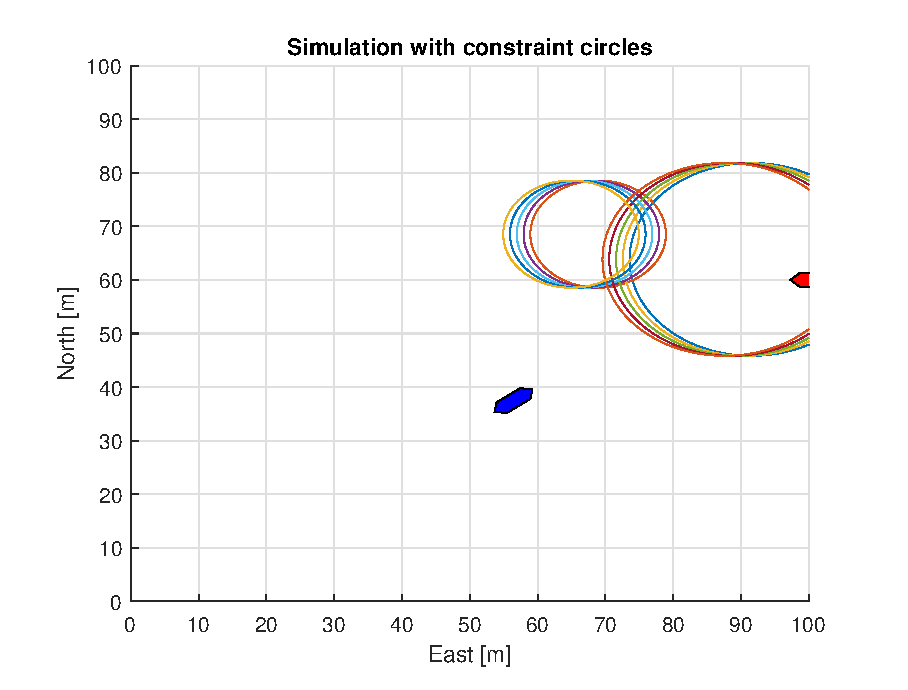
\includegraphics[width=\textwidth]{Images/Figures/Enkel_GW/Simple0_f1_Frame3}
        \subcaption{caption}
    \end{subfigure}
    \hfill
    \begin{subfigure}[b]{0.499\textwidth}
        \centering
        \includegraphics[width=\textwidth]{Images/Figures/Enkel_GW/Simple0_f600_Frame3}
        \subcaption{mhm}
    \end{subfigure}
    \hfill
\end{figure}% 
\begin{figure}[ht]\ContinuedFloat
    \begin{subfigure}[b]{0.49\textwidth}
        \centering
        \includegraphics[width=\textwidth]{Images/Figures/Enkel_GW/Simple0_f1_Frame4}
        \subcaption{caption}
    \end{subfigure}
    \hfill
    \begin{subfigure}[b]{0.499\textwidth}
        \centering
        \includegraphics[width=\textwidth]{Images/Figures/Enkel_GW/Simple0_f600_Frame4}
        \subcaption{mhm}
    \end{subfigure}
    \hfill
    \\
    \begin{subfigure}[b]{0.49\textwidth}
        \centering
        \includegraphics[width=\textwidth]{Images/Figures/Enkel_GW/Simple0_f1_Frame5}
        \subcaption{caption}
    \end{subfigure}
    \hfill
    \begin{subfigure}[b]{0.499\textwidth}
        \centering
        \includegraphics[width=\textwidth]{Images/Figures/Enkel_GW/Simple0_f600_Frame5}
        \subcaption{mhm}
    \end{subfigure}
    \hfill
    \caption{TODO: Skriv. Enkel GW sim med og uten constraints}
\end{figure}

\begin{figure} %w\_opt for Enkel GW
    \begin{subfigure}[b]{0.49\textwidth}
        \centering
        \includegraphics[width=\textwidth]{Images/Figures/Enkel_GW/Simple0_f999_Frame1}
        \subcaption{caption}
    \end{subfigure}
    \hfill
    \begin{subfigure}[b]{0.499\textwidth}
        \centering
        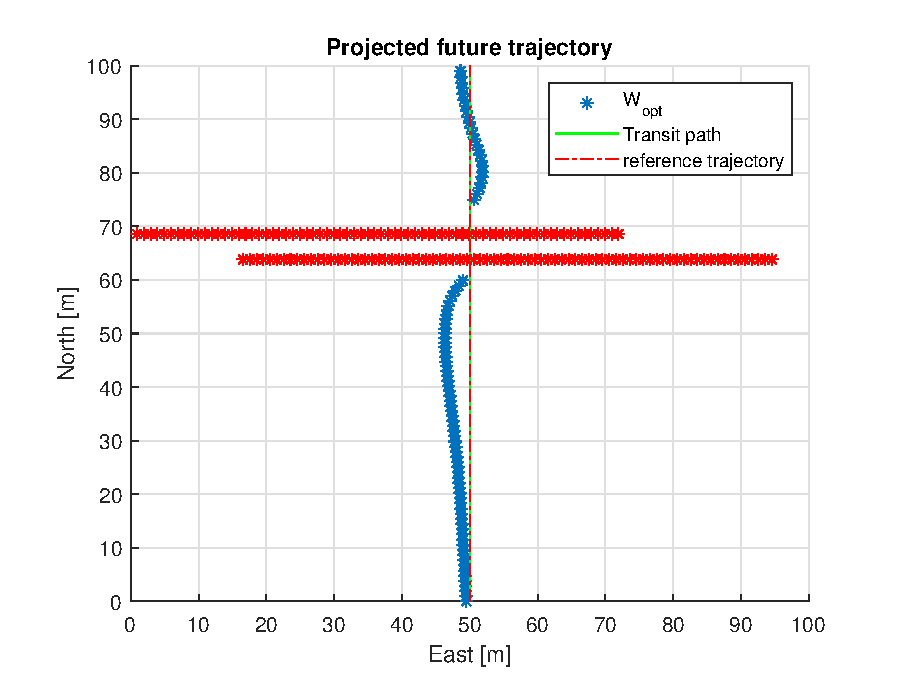
\includegraphics[width=\textwidth]{Images/Figures/Enkel_GW/Simple0_f999_Frame2}
        \subcaption{mhm}
    \end{subfigure}
    \hfill
    \\
    \begin{subfigure}[b]{0.49\textwidth}
        \centering
        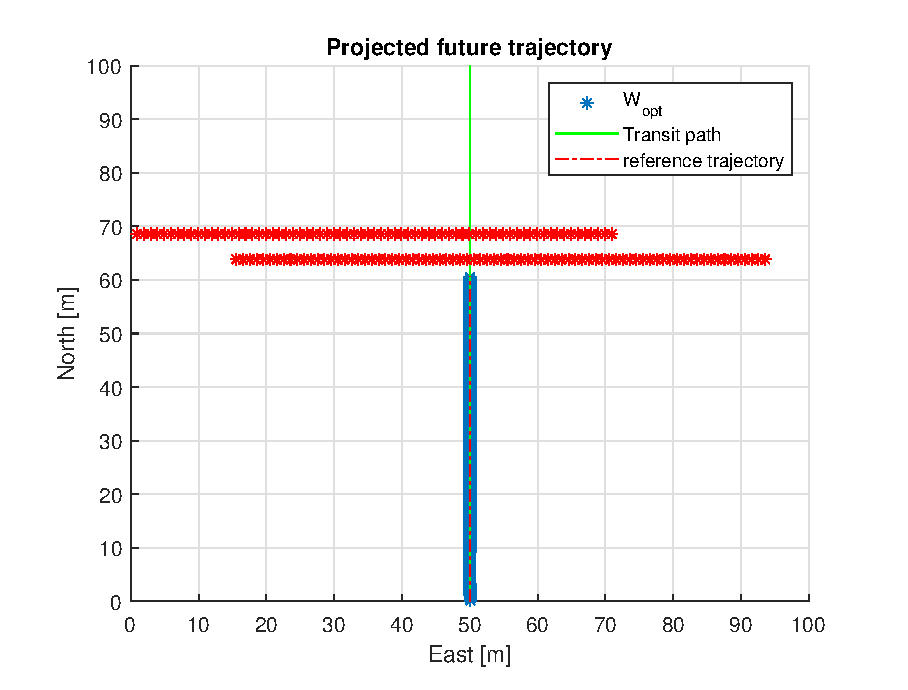
\includegraphics[width=\textwidth]{Images/Figures/Enkel_GW/Simple0_f999_Frame3}
        \subcaption{caption}
    \end{subfigure}
    \hfill
    \begin{subfigure}[b]{0.499\textwidth}
        \centering
        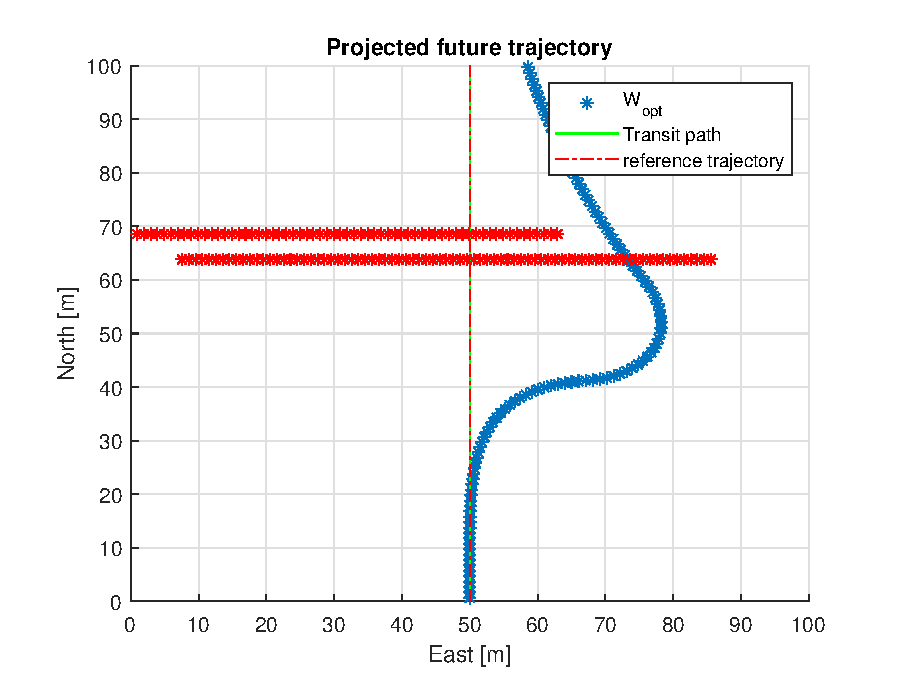
\includegraphics[width=\textwidth]{Images/Figures/Enkel_GW/Simple0_f999_Frame4}
        \subcaption{mhm}
    \end{subfigure}
    \hfill
    \\
    \begin{subfigure}[b]{0.49\textwidth}
        \centering
        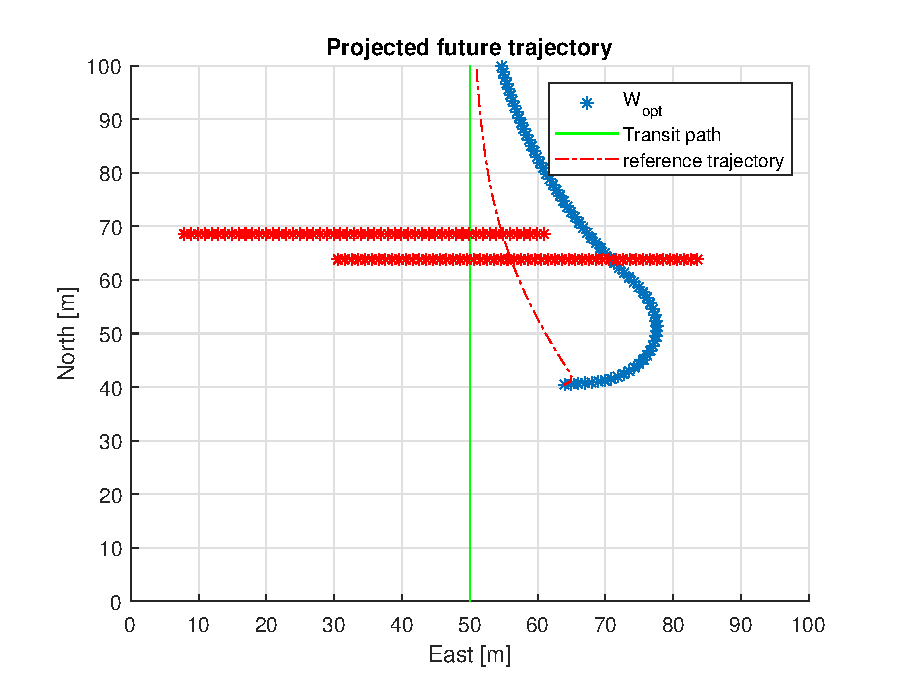
\includegraphics[width=\textwidth]{Images/Figures/Enkel_GW/Simple0_f999_Frame5}
        \subcaption{caption}
    \end{subfigure}
    \hfill
    \begin{subfigure}[b]{0.499\textwidth}
        \centering
        \includegraphics[width=\textwidth]{Images/Figures/Enkel_GW/simple0_f999_Frame6}
        \subcaption{mhm}
    \end{subfigure}
    \hfill
    \caption{w\_opt for Enkel GW}
\end{figure}

\subsubsection{Simple Stand On}
\begin{figure}[!b] %Enkel SO
    \begin{subfigure}[b]{0.49\textwidth}
        \centering
        \includegraphics[width=\textwidth]{Images/Figures/Enkel_SO/Simple0_f1_Frame1}
        \subcaption{caption}
    \end{subfigure}
    \hfill
    \begin{subfigure}[b]{0.499\textwidth}
        \centering
        \includegraphics[width=\textwidth]{Images/Figures/Enkel_SO/Simple0_f600_Frame1}
        \subcaption{mhm}
    \end{subfigure}
    \hfill
    \\
    \begin{subfigure}[b]{0.49\textwidth}
        \centering
        \includegraphics[width=\textwidth]{Images/Figures/Enkel_SO/Simple0_f1_Frame2}
        \subcaption{caption}
    \end{subfigure}
    \hfill
    \begin{subfigure}[b]{0.499\textwidth}
        \centering
        \includegraphics[width=\textwidth]{Images/Figures/Enkel_SO/Simple0_f600_Frame2}
        \subcaption{mhm}
    \end{subfigure}
    \hfill
    \\
    \begin{subfigure}[b]{0.49\textwidth}
        \centering
        \includegraphics[width=\textwidth]{Images/Figures/Enkel_SO/Simple0_f1_Frame3}
        \subcaption{caption}
    \end{subfigure}
    \hfill
    \begin{subfigure}[b]{0.499\textwidth}
        \centering
        \includegraphics[width=\textwidth]{Images/Figures/Enkel_SO/Simple0_f600_Frame3}
        \subcaption{mhm}
    \end{subfigure}
    \hfill
    \caption{Enkel SO}
\end{figure}% 

\begin{figure} %w\_opt for Enkel SO
    \begin{subfigure}[b]{0.49\textwidth}
        \centering
        \includegraphics[width=\textwidth]{Images/Figures/Enkel_SO/Simple0_f999_Frame1}
        \subcaption{caption}
    \end{subfigure}
    \hfill
    \begin{subfigure}[b]{0.499\textwidth}
        \centering
        \includegraphics[width=\textwidth]{Images/Figures/Enkel_SO/Simple0_f999_Frame2}
        \subcaption{mhm}
    \end{subfigure}
    \hfill
    \\
    \begin{subfigure}[b]{0.49\textwidth}
        \centering
        \includegraphics[width=\textwidth]{Images/Figures/Enkel_SO/Simple0_f999_Frame3}
        \subcaption{caption}
    \end{subfigure}
    \hfill
    \begin{subfigure}[b]{0.499\textwidth}
        \centering
        \includegraphics[width=\textwidth]{Images/Figures/Enkel_SO/Simple0_f999_Frame4}
        \subcaption{mhm}
    \end{subfigure}
    \hfill
    \caption{w\_opt for Enkel SO}
\end{figure}


\subsubsection{Turn Head On}
\clearpage
\begin{figure}[!b] %TODO: Skriv. Sving HO sim med og uten constraints
    \begin{subfigure}[b]{0.49\textwidth}
        \centering
        \includegraphics[width=\textwidth]{Images/Figures/sving_HO/Simple0_f1_Frame1}
        \subcaption{caption}
    \end{subfigure}
    \hfill
    \begin{subfigure}[b]{0.499\textwidth}
        \centering
        \includegraphics[width=\textwidth]{Images/Figures/sving_HO/Simple0_f600_Frame1}
        \subcaption{mhm}
    \end{subfigure}
    \hfill
    \\
    \begin{subfigure}[b]{0.49\textwidth}
        \centering
        \includegraphics[width=\textwidth]{Images/Figures/sving_HO/Simple0_f1_Frame2}
        \subcaption{caption}
    \end{subfigure}
    \hfill
    \begin{subfigure}[b]{0.499\textwidth}
        \centering
        \includegraphics[width=\textwidth]{Images/Figures/sving_HO/Simple0_f600_Frame2}
        \subcaption{mhm}
    \end{subfigure}
    \hfill
    \\
    \begin{subfigure}[b]{0.49\textwidth}
        \centering
        \includegraphics[width=\textwidth]{Images/Figures/sving_HO/Simple0_f1_Frame3}
        \subcaption{caption}
    \end{subfigure}
    \hfill
    \begin{subfigure}[b]{0.499\textwidth}
        \centering
        \includegraphics[width=\textwidth]{Images/Figures/sving_HO/Simple0_f600_Frame3}
        \subcaption{mhm}
    \end{subfigure}
    \hfill
\end{figure}% 
\begin{figure}[ht]\ContinuedFloat
    \begin{subfigure}[b]{0.49\textwidth}
        \centering
        \includegraphics[width=\textwidth]{Images/Figures/sving_HO/Simple0_f1_Frame4}
        \subcaption{caption}
    \end{subfigure}
    \hfill
    \begin{subfigure}[b]{0.499\textwidth}
        \centering
        \includegraphics[width=\textwidth]{Images/Figures/sving_HO/Simple0_f600_Frame4}
        \subcaption{mhm}
    \end{subfigure}
    \hfill
    \\
    \begin{subfigure}[b]{0.49\textwidth}
        \centering
        \includegraphics[width=\textwidth]{Images/Figures/sving_HO/Simple0_f1_Frame5}
        \subcaption{caption}
    \end{subfigure}
    \hfill
    \begin{subfigure}[b]{0.499\textwidth}
        \centering
        \includegraphics[width=\textwidth]{Images/Figures/sving_HO/Simple0_f600_Frame5}
        \subcaption{mhm}
    \end{subfigure}
    \hfill
    \caption{TODO: Skriv. Sving HO sim med og uten constraints}
\end{figure}

\begin{figure} %w\_opt for Sving HO
    \begin{subfigure}[b]{0.49\textwidth}
        \centering
        \includegraphics[width=\textwidth]{Images/Figures/sving_HO/Simple0_f999_Frame1}
        \subcaption{caption}
    \end{subfigure}
    \hfill
    \begin{subfigure}[b]{0.499\textwidth}
        \centering
        \includegraphics[width=\textwidth]{Images/Figures/sving_HO/Simple0_f999_Frame2}
        \subcaption{mhm}
    \end{subfigure}
    \hfill
    \\
    \begin{subfigure}[b]{0.49\textwidth}
        \centering
        \includegraphics[width=\textwidth]{Images/Figures/sving_HO/Simple0_f999_Frame3}
        \subcaption{caption}
    \end{subfigure}
    \hfill
    \begin{subfigure}[b]{0.499\textwidth}
        \centering
        \includegraphics[width=\textwidth]{Images/Figures/sving_HO/Simple0_f999_Frame4}
        \subcaption{mhm}
    \end{subfigure}
    \hfill
    \begin{subfigure}[b]{0.5\textwidth}
        \centering
        \includegraphics[width=\textwidth]{Images/Figures/Sving_HO/simple0_f999_frame5}
        \subcaption{mhm}
    \end{subfigure}
    \caption{w\_opt for Sving HO}
\end{figure}


\subsubsection{Turn Give Way}
%% WITH PREDICTIOn
\clearpage
\begin{figure}[!b] % TODO: Skriv. Sving GW sim med og uten constraints AND WITH PREDICTION
    \begin{subfigure}[b]{0.49\textwidth}
        \centering
        \includegraphics[width=\textwidth]{Images/Figures/sving_GW/Simple0_f1_Frame1}
        \subcaption{caption}
    \end{subfigure}
    \hfill
    \begin{subfigure}[b]{0.499\textwidth}
        \centering
        \includegraphics[width=\textwidth]{Images/Figures/sving_GW/Simple0_f600_Frame1}
        \subcaption{mhm}
    \end{subfigure}
    \hfill
    \\
    \begin{subfigure}[b]{0.49\textwidth}
        \centering
        \includegraphics[width=\textwidth]{Images/Figures/sving_GW/Simple0_f1_Frame2}
        \subcaption{caption}
    \end{subfigure}
    \hfill
    \begin{subfigure}[b]{0.499\textwidth}
        \centering
        \includegraphics[width=\textwidth]{Images/Figures/sving_GW/Simple0_f600_Frame2}
        \subcaption{mhm}
    \end{subfigure}
    \hfill
    \\
    \begin{subfigure}[b]{0.49\textwidth}
        \centering
        \includegraphics[width=\textwidth]{Images/Figures/sving_GW/Simple0_f1_Frame3}
        \subcaption{caption}
    \end{subfigure}
    \hfill
    \begin{subfigure}[b]{0.499\textwidth}
        \centering
        \includegraphics[width=\textwidth]{Images/Figures/sving_GW/Simple0_f600_Frame3}
        \subcaption{mhm}
    \end{subfigure}
    \hfill
\end{figure}% 
\begin{figure}[ht]\ContinuedFloat
    \begin{subfigure}[b]{0.49\textwidth}
        \centering
        \includegraphics[width=\textwidth]{Images/Figures/sving_GW/Simple0_f1_Frame4}
        \subcaption{caption}
    \end{subfigure}
    \hfill
    \begin{subfigure}[b]{0.499\textwidth}
        \centering
        \includegraphics[width=\textwidth]{Images/Figures/sving_GW/Simple0_f600_Frame4}
        \subcaption{mhm}
    \end{subfigure}
    \hfill
    \\
    \begin{subfigure}[b]{0.49\textwidth}
        \centering
        \includegraphics[width=\textwidth]{Images/Figures/sving_GW/Simple0_f1_Frame5}
        \subcaption{caption}
    \end{subfigure}
    \hfill
    \begin{subfigure}[b]{0.499\textwidth}
        \centering
        \includegraphics[width=\textwidth]{Images/Figures/sving_GW/Simple0_f600_Frame5}
        \subcaption{mhm}
    \end{subfigure}
    \hfill
    \\
    \begin{subfigure}[b]{0.49\textwidth}
        \centering
        \includegraphics[width=\textwidth]{Images/Figures/sving_GW/Simple0_f1_Frame6}
        \subcaption{caption}
    \end{subfigure}
    \hfill
    \begin{subfigure}[b]{0.499\textwidth}
        \centering
        \includegraphics[width=\textwidth]{Images/Figures/sving_GW/Simple0_f600_Frame6}
        \subcaption{mhm}
    \end{subfigure}
    \hfill
    \caption{TODO: Skriv. Sving GW sim med og uten constraints AND WITH PREDICTION}
\end{figure}

\begin{figure} %w\_opt for Sving GW WITH PREDICTION
    \begin{subfigure}[b]{0.49\textwidth}
        \centering
        \includegraphics[width=\textwidth]{Images/Figures/sving_GW/Simple0_f999_Frame1}
        \subcaption{caption}
    \end{subfigure}
    \hfill
    \begin{subfigure}[b]{0.499\textwidth}
        \centering
        \includegraphics[width=\textwidth]{Images/Figures/sving_GW/Simple0_f999_Frame2}
        \subcaption{mhm}
    \end{subfigure}
    \hfill
    \\
    \begin{subfigure}[b]{0.49\textwidth}
        \centering
        \includegraphics[width=\textwidth]{Images/Figures/sving_GW/Simple0_f999_Frame3}
        \subcaption{caption}
    \end{subfigure}
    \hfill
    \begin{subfigure}[b]{0.499\textwidth}
        \centering
        \includegraphics[width=\textwidth]{Images/Figures/sving_GW/Simple0_f999_Frame4}
        \subcaption{mhm}
    \end{subfigure}
    \hfill
    \\
    \begin{subfigure}[b]{0.49\textwidth}
        \centering
        \includegraphics[width=\textwidth]{Images/Figures/sving_GW/simple0_f999_frame5}
        \subcaption{mhm}
    \end{subfigure}
    \hfill
    \begin{subfigure}[b]{0.49\textwidth}
        \centering
        \includegraphics[width=\textwidth]{Images/Figures/sving_GW/simple0_f999_frame6}
        \subcaption{mhm}
    \end{subfigure}
    \caption{w\_opt for Sving GW WITH PREDICTION}
\end{figure} 


%% WITHOUT PREDICTION
\clearpage
\begin{figure}[!b] %TODO: Skriv. Sving GW sim med og uten constraints AND WITHOUT PREDICTION
    \begin{subfigure}[b]{0.49\textwidth}
        \centering
        \includegraphics[width=\textwidth]{Images/Figures/sving_GW/Simple1_f1_Frame1}
        \subcaption{caption}
    \end{subfigure}
    \hfill
    \begin{subfigure}[b]{0.499\textwidth}
        \centering
        \includegraphics[width=\textwidth]{Images/Figures/sving_GW/Simple1_f600_Frame1}
        \subcaption{mhm}
    \end{subfigure}
    \hfill
    \\
    \begin{subfigure}[b]{0.49\textwidth}
        \centering
        \includegraphics[width=\textwidth]{Images/Figures/sving_GW/Simple1_f1_Frame2}
        \subcaption{caption}
    \end{subfigure}
    \hfill
    \begin{subfigure}[b]{0.499\textwidth}
        \centering
        \includegraphics[width=\textwidth]{Images/Figures/sving_GW/Simple1_f600_Frame2}
        \subcaption{mhm}
    \end{subfigure}
    \hfill
    \\
    \begin{subfigure}[b]{0.49\textwidth}
        \centering
        \includegraphics[width=\textwidth]{Images/Figures/sving_GW/Simple1_f1_Frame3}
        \subcaption{caption}
    \end{subfigure}
    \hfill
    \begin{subfigure}[b]{0.499\textwidth}
        \centering
        \includegraphics[width=\textwidth]{Images/Figures/sving_GW/Simple1_f600_Frame3}
        \subcaption{mhm}
    \end{subfigure}
    \hfill
\end{figure}% 
\begin{figure}[ht]\ContinuedFloat
    \begin{subfigure}[b]{0.49\textwidth}
        \centering
        \includegraphics[width=\textwidth]{Images/Figures/sving_GW/Simple1_f1_Frame4}
        \subcaption{caption}
    \end{subfigure}
    \hfill
    \begin{subfigure}[b]{0.499\textwidth}
        \centering
        \includegraphics[width=\textwidth]{Images/Figures/sving_GW/Simple1_f600_Frame4}
        \subcaption{mhm}
    \end{subfigure}
    \hfill
    \\
    \begin{subfigure}[b]{0.49\textwidth}
        \centering
        \includegraphics[width=\textwidth]{Images/Figures/sving_GW/Simple1_f1_Frame5}
        \subcaption{caption}
    \end{subfigure}
    \hfill
    \begin{subfigure}[b]{0.499\textwidth}
        \centering
        \includegraphics[width=\textwidth]{Images/Figures/sving_GW/Simple1_f600_Frame5}
        \subcaption{mhm}
    \end{subfigure}
    \hfill
    \\
    \begin{subfigure}[b]{0.49\textwidth}
        \centering
        \includegraphics[width=\textwidth]{Images/Figures/sving_GW/Simple1_f1_Frame6}
        \subcaption{caption}
    \end{subfigure}
    \hfill
    \begin{subfigure}[b]{0.499\textwidth}
        \centering
        \includegraphics[width=\textwidth]{Images/Figures/sving_GW/Simple1_f600_Frame6}
        \subcaption{mhm}
    \end{subfigure}
    \hfill
    \caption{TODO: Skriv. Sving GW sim med og uten constraints AND WITHOUT PREDICTION}
\end{figure}

\begin{figure} % w\_opt for Sving GW WITHOUT PREDICTION
    \begin{subfigure}[b]{0.49\textwidth}
        \centering
        \includegraphics[width=\textwidth]{Images/Figures/sving_GW/Simple1_f999_Frame1}
        \subcaption{caption}
    \end{subfigure}
    \hfill
    \begin{subfigure}[b]{0.499\textwidth}
        \centering
        \includegraphics[width=\textwidth]{Images/Figures/sving_GW/Simple1_f999_Frame2}
        \subcaption{mhm}
    \end{subfigure}
    \hfill
    \\
    \begin{subfigure}[b]{0.49\textwidth}
        \centering
        \includegraphics[width=\textwidth]{Images/Figures/sving_GW/Simple1_f999_Frame3}
        \subcaption{caption}
    \end{subfigure}
    \hfill
    \begin{subfigure}[b]{0.499\textwidth}
        \centering
        \includegraphics[width=\textwidth]{Images/Figures/sving_GW/Simple1_f999_Frame4}
        \subcaption{mhm}
    \end{subfigure}
    \hfill
    \\
    \begin{subfigure}[b]{0.49\textwidth}
        \centering
        \includegraphics[width=\textwidth]{Images/Figures/sving_GW/simple1_f999_frame5}
        \subcaption{mhm}
    \end{subfigure}
    \hfill
    \begin{subfigure}[b]{0.49\textwidth}
        \centering
        \includegraphics[width=\textwidth]{Images/Figures/sving_GW/simple1_f999_frame6}
        \subcaption{mhm}
    \end{subfigure}
    \caption{w\_opt for Sving GW WITHOUT PREDICTION}
\end{figure} 


\subsubsection{Turn Stand On}
\clearpage
\begin{figure}[!b] %TODO: Sving SO med og uten constraints
    \begin{subfigure}[b]{0.49\textwidth}
        \centering
        \includegraphics[width=\textwidth]{Images/Figures/sving_SO/Simple0_f1_Frame1}
        \subcaption{caption}
    \end{subfigure}
    \hfill
    \begin{subfigure}[b]{0.499\textwidth}
        \centering
        \includegraphics[width=\textwidth]{Images/Figures/sving_SO/Simple0_f600_Frame1}
        \subcaption{mhm}
    \end{subfigure}
    \hfill
    \\
    \begin{subfigure}[b]{0.49\textwidth}
        \centering
        \includegraphics[width=\textwidth]{Images/Figures/sving_SO/Simple0_f1_Frame2}
        \subcaption{caption}
    \end{subfigure}
    \hfill
    \begin{subfigure}[b]{0.499\textwidth}
        \centering
        \includegraphics[width=\textwidth]{Images/Figures/sving_SO/Simple0_f600_Frame2}
        \subcaption{mhm}
    \end{subfigure}
    \hfill
    \\
    \begin{subfigure}[b]{0.49\textwidth}
        \centering
        \includegraphics[width=\textwidth]{Images/Figures/sving_SO/Simple0_f1_Frame3}
        \subcaption{caption}
    \end{subfigure}
    \hfill
    \begin{subfigure}[b]{0.499\textwidth}
        \centering
        \includegraphics[width=\textwidth]{Images/Figures/sving_SO/Simple0_f600_Frame3}
        \subcaption{mhm}
    \end{subfigure}
    \hfill
\end{figure}% 
\begin{figure}[ht]\ContinuedFloat
    \begin{subfigure}[b]{0.49\textwidth}
        \centering
        \includegraphics[width=\textwidth]{Images/Figures/sving_SO/Simple0_f1_Frame4}
        \subcaption{caption}
    \end{subfigure}
    \hfill
    \begin{subfigure}[b]{0.499\textwidth}
        \centering
        \includegraphics[width=\textwidth]{Images/Figures/sving_SO/Simple0_f600_Frame4}
        \subcaption{mhm}
    \end{subfigure}
    \caption{TODO: Sving SO med og uten constraints}
\end{figure}

\begin{figure} %w\_opt for Sving SO with prediction
    \begin{subfigure}[b]{0.49\textwidth}
        \centering
        \includegraphics[width=\textwidth]{Images/Figures/sving_SO/Simple0_f999_Frame1}
        \subcaption{caption}
    \end{subfigure}
    \hfill
    \begin{subfigure}[b]{0.499\textwidth}
        \centering
        \includegraphics[width=\textwidth]{Images/Figures/sving_SO/Simple0_f999_Frame2}
        \subcaption{mhm}
    \end{subfigure}
    \hfill
    \\
    \begin{subfigure}[b]{0.49\textwidth}
        \centering
        \includegraphics[width=\textwidth]{Images/Figures/sving_SO/Simple0_f999_Frame3}
        \subcaption{caption}
    \end{subfigure}
    \hfill
    \begin{subfigure}[b]{0.499\textwidth}
        \centering
        \includegraphics[width=\textwidth]{Images/Figures/sving_SO/Simple0_f999_Frame4}
        \subcaption{mhm}
    \end{subfigure}
    \caption{w\_opt for Sving SO with prediction}
\end{figure}

\subsubsection{Canals}
\begin{itemize}
    \item blocked path
    \item feasibility check
    \item forskjell mellom prediction metoder
\end{itemize}


%% Canals With Prediction
\clearpage
\begin{figure}[!b] %Canals simulation, shown with and without constraints
    \begin{subfigure}[b]{0.49\textwidth}
        \centering
        \includegraphics[width=\textwidth]{Images/Figures/Havn1/Simple0_f1_Frame1}
        \subcaption{caption}
    \end{subfigure}
    \hfill
    \begin{subfigure}[b]{0.499\textwidth}
        \centering
        \includegraphics[width=\textwidth]{Images/Figures/Havn1/Simple0_f600_Frame1}
        \subcaption{mhm}
    \end{subfigure}
    \hfill
    \\
    \begin{subfigure}[b]{0.49\textwidth}
        \centering
        \includegraphics[width=\textwidth]{Images/Figures/Havn1/Simple0_f1_Frame2}
        \subcaption{caption}
    \end{subfigure}
    \hfill
    \begin{subfigure}[b]{0.499\textwidth}
        \centering
        \includegraphics[width=\textwidth]{Images/Figures/Havn1/Simple0_f600_Frame2}
        \subcaption{mhm}
    \end{subfigure}
    \hfill
    \\
    \begin{subfigure}[b]{0.49\textwidth}
        \centering
        \includegraphics[width=\textwidth]{Images/Figures/Havn1/Simple0_f1_Frame3}
        \subcaption{caption}
    \end{subfigure}
    \hfill
    \begin{subfigure}[b]{0.499\textwidth}
        \centering
        \includegraphics[width=\textwidth]{Images/Figures/Havn1/Simple0_f600_Frame3}
        \subcaption{mhm}
    \end{subfigure}
    \hfill
\end{figure}%
\begin{figure}[ht]\ContinuedFloat
    \begin{subfigure}[b]{0.49\textwidth}
        \centering
        \includegraphics[width=\textwidth]{Images/Figures/Havn1/Simple0_f1_Frame4}
        \subcaption{caption}
    \end{subfigure}
    \hfill
    \begin{subfigure}[b]{0.499\textwidth}
        \centering
        \includegraphics[width=\textwidth]{Images/Figures/Havn1/Simple0_f600_Frame4}
        \subcaption{mhm}
    \end{subfigure}
    \hfill
    \\
    \begin{subfigure}[b]{0.49\textwidth}
        \centering
        \includegraphics[width=\textwidth]{Images/Figures/Havn1/Simple0_f1_Frame5}
        \subcaption{caption}
    \end{subfigure}
    \hfill
    \begin{subfigure}[b]{0.499\textwidth}
        \centering
        \includegraphics[width=\textwidth]{Images/Figures/Havn1/Simple0_f600_Frame5}
        \subcaption{mhm}
    \end{subfigure}
    \hfill
    \caption{Canals simulation, shown with and without constraints}
\end{figure}

\begin{figure} %Predicted path over the course of the Canals simulation
    \begin{subfigure}[b]{0.49\textwidth}
        \centering
        \includegraphics[width=\textwidth]{Images/Figures/Havn1/Simple0_f999_Frame1}
        \subcaption{caption}
    \end{subfigure}
    \hfill
    \begin{subfigure}[b]{0.499\textwidth}
        \centering
        \includegraphics[width=\textwidth]{Images/Figures/Havn1/Simple0_f999_Frame2}
        \subcaption{mhm}
    \end{subfigure}
    \hfill
    \\
    \begin{subfigure}[b]{0.49\textwidth}
        \centering
        \includegraphics[width=\textwidth]{Images/Figures/Havn1/Simple0_f999_Frame3}
        \subcaption{caption}
    \end{subfigure}
    \hfill
    \begin{subfigure}[b]{0.499\textwidth}
        \centering
        \includegraphics[width=\textwidth]{Images/Figures/Havn1/Simple0_f999_Frame4}
        \subcaption{mhm}
    \end{subfigure}
    \hfill
    \\
    \begin{subfigure}[b]{0.49\textwidth}
        \centering
        \includegraphics[width=\textwidth]{Images/Figures/Havn1/Simple0_f999_Frame5}
        \subcaption{caption}
    \end{subfigure}
    \hfill
    \begin{subfigure}[b]{0.499\textwidth}
        \centering
        \includegraphics[width=\textwidth]{Images/Figures/Havn1/Simple0_f999_Frame6}
        \subcaption{mhm}
    \end{subfigure}
    \hfill
    \caption{Predicted path over the course of the Canals simulation}
\end{figure}


%%C Canals Without Prediction
\clearpage
\begin{figure}[!b] %Canals simulation without prediction, shown with and without constraints
    \begin{subfigure}[b]{0.49\textwidth}
        \centering
        \includegraphics[width=\textwidth]{Images/Figures/Havn1/Simple1_f1_Frame1}
        \caption{caption}
    \end{subfigure}
    \hfill
    \begin{subfigure}[b]{0.499\textwidth}
        \centering
        \includegraphics[width=\textwidth]{Images/Figures/Havn1/Simple1_f600_Frame1}
        \caption{mhm}
    \end{subfigure}
    \hfill
    \\
    \begin{subfigure}[b]{0.49\textwidth}
        \centering
        \includegraphics[width=\textwidth]{Images/Figures/Havn1/Simple1_f1_Frame2}
        \caption{caption}
    \end{subfigure}
    \hfill
    \begin{subfigure}[b]{0.499\textwidth}
        \centering
        \includegraphics[width=\textwidth]{Images/Figures/Havn1/Simple1_f600_Frame2}
        \caption{mhm}
    \end{subfigure}
    \hfill
    \\
    \begin{subfigure}[b]{0.49\textwidth}
        \centering
        \includegraphics[width=\textwidth]{Images/Figures/Havn1/Simple1_f1_Frame3}
        \caption{caption}
    \end{subfigure}
    \hfill
    \begin{subfigure}[b]{0.499\textwidth}
        \centering
        \includegraphics[width=\textwidth]{Images/Figures/Havn1/Simple1_f600_Frame3}
        \caption{mhm}
    \end{subfigure}
    \hfill
\end{figure}%
\begin{figure}[ht]\ContinuedFloat
    \begin{subfigure}[b]{0.49\textwidth}
        \centering
        \includegraphics[width=\textwidth]{Images/Figures/Havn1/Simple1_f1_Frame5}
        \subcaption{dsadada}
    \end{subfigure}
    \hfill
    \begin{subfigure}[b]{0.499\textwidth}
        \centering
        \includegraphics[width=\textwidth]{Images/Figures/Havn1/Simple1_f600_Frame5}
        \subcaption{mhm}
    \end{subfigure}
    \hfill
    \\
    \begin{subfigure}[b]{0.49\textwidth}
        \centering
        \includegraphics[width=\textwidth]{Images/Figures/Havn1/Simple1_f1_Frame6}
        \subcaption{caption}
    \end{subfigure}
    \hfill
    \begin{subfigure}[b]{0.499\textwidth}
        \centering
        \includegraphics[width=\textwidth]{Images/Figures/Havn1/Simple1_f600_Frame6}
        \subcaption{mhm}
    \end{subfigure}
    \hfill
    \\
    \begin{subfigure}[b]{0.49\textwidth}
        \centering
        \includegraphics[width=\textwidth]{Images/Figures/Havn1/Simple1_f1_Frame7}
        \subcaption{caption}
    \end{subfigure}
    \hfill
    \begin{subfigure}[b]{0.499\textwidth}
        \centering
        \includegraphics[width=\textwidth]{Images/Figures/Havn1/Simple1_f600_Frame7}
        \subcaption{mhm}
    \end{subfigure}
    \hfill
    \caption{Canals simulation without prediction, shown with and without constraints}
\end{figure}

\begin{figure} % TODO: skriv. Havn1 w\_opt without prediction
    \begin{subfigure}[b]{0.49\textwidth}
        \centering
        \includegraphics[width=\textwidth]{Images/Figures/Havn1/Simple1_f999_Frame1}
        \subcaption{caption}
    \end{subfigure}
    \hfill
    \begin{subfigure}[b]{0.499\textwidth}
        \centering
        \includegraphics[width=\textwidth]{Images/Figures/Havn1/Simple1_f999_Frame2}
        \subcaption{mhm}
    \end{subfigure}
    \hfill
    \\
    \begin{subfigure}[b]{0.49\textwidth}
        \centering
        \includegraphics[width=\textwidth]{Images/Figures/Havn1/Simple1_f999_Frame3}
        \subcaption{caption}
    \end{subfigure}
    \hfill
    \begin{subfigure}[b]{0.499\textwidth}
        \centering
        \includegraphics[width=\textwidth]{Images/Figures/Havn1/Simple1_f999_Frame5}
        \subcaption{mhm}
    \end{subfigure}
    \hfill
    \\
    \begin{subfigure}[b]{0.49\textwidth}
        \centering
        \includegraphics[width=\textwidth]{Images/Figures/Havn1/Simple1_f999_Frame6}
        \subcaption{caption}
    \end{subfigure}
    \hfill
    \begin{subfigure}[b]{0.499\textwidth}
        \centering
        \includegraphics[width=\textwidth]{Images/Figures/Havn1/Simple1_f999_Frame7}
        \subcaption{mhm}
    \end{subfigure}
    \hfill
    \caption{TODO: skriv. Havn1 w\_opt without prediction}
\end{figure}


\subsubsection{Helløya}
(TODO: Skriv og figurer)

\subsubsection{Skjærgård}
(TODO: Skriv og figurer)

\subsubsection{Trondheimsfjord}
(TODO: Skriv og figurer.)

\subsubsection{Miscellaneous}
\begin{itemize}
    \item Bad Prediction, what happens when the target ship does not follow the predicted path
    \item Blocked Path, a closer look at what happens when the path we intend to take is fully blocked.
    \item Wrong turn, observe that the optimal trajectory is often to turn the wrong direction slightly when changing course.
    \item WrapTo2Pi problems, how to explain to an algorithm how course works.
    \item 'Dragged' along by Target Ships. When does it happen.
\end{itemize}

\begin{figure} %TODO: Skriv om bad prediction
    \centering
    \begin{subfigure}[b]{0.45\textwidth}
        \centering
        \includegraphics[width=\textwidth]{Images/BadPrediction_Caught_in_constraints.pdf}
        \subcaption{TODO: SKriv. when prediction is poorly executed the risk of getting entangled in constraints increases.}
    \end{subfigure}
    \hfill 
    \begin{subfigure}[b]{0.45\textwidth}
        \centering
        \includegraphics[width=\textwidth]{images/BadPrediction_w_opt.pdf}
        \subcaption{TODO: Skriv. When entangled in constraints the solver is unable to find a feasible solution.}
    \end{subfigure}
    \caption{TODO: Skriv om bad prediction}
\end{figure}


\begin{figure} %TODO: A blocked path event, and how the solution develops
    \centering
    \begin{subfigure}[b]{0.61\textwidth}
        \centering
        \includegraphics[width=\textwidth]{Images/Completely_Blocked.pdf}
        \subcaption{TODO: SKriv. A Target ship is predicted to completely block our path}
    \end{subfigure}
    \hfill 
    \begin{subfigure}[b]{0.61\textwidth}
        \centering
        \includegraphics[width=\textwidth]{images/Completely_blocked_wopt.pdf}
        \subcaption{TODO: Skriv. When the path is blocked, the solution will never be feasible.}
    \end{subfigure}
    \hfill
    \begin{subfigure}[b]{0.61\textwidth}
        \centering
        \includegraphics[width=\textwidth]{images/Completely_blocked_wopt_next.pdf}
        \subcaption{TODO: Skriv. The solution for the next iteration, when speed is reduced by a factor of 3}
    \end{subfigure}
    \caption{TODO: A blocked path event, and how the solution develops}
\end{figure}
%\subsection{Fullscale Testing}
%\begin{itemize}
%    \item Hvorfor fullskalatester.
%    \item Hva Skal testes.
%    \item Hva er det jeg håper fullskalatest vil vise oss.
%    \item Hvis jeg ikke skriver om hvordan jeg implementerer kode og gjennomfører testene i metode kapittelet så må det beskrives her.
%    \item Kriterier som skal testes?
%\end{itemize}

%\subsection{Fullscale Test Results}
%\begin{itemize}
%    \item Skriv om hvordan det gikk.
%\end{itemize}

\subsection{Discussion}
\begin{itemize}
    \item Hvorfor er viktigere en hva
    \item ikke overanalyser resultat, ikke dra ville konklusjoner.
    \item Hvis et resultat er mye værre enn forventet kan det godt være det er bugs.
    \item i tillegg til det resultatene viser kan jeg også skrive om det jeg kan se med debugging.
    \item WrapTo2Pi problems (shortest signed angle stuff)
    \item Turning the wrong way to get a more even turn, Optimization leads to this problem. 
\end{itemize}

\subsection{Improvements over previous version}
\begin{itemize}
    \item Definite improvements in terms of computational efficiency. This greatly increases the likelyhood of finding an optimal solution 
    \item Because of the better efficiency the algorithm is also able to handle more control intervals, This means it is better at handling both greater time horizon and shorter control interval steps.
    \item The new method for handling static obstacles is much less prone to misplaced or inefficnet constraints. (her ta gjerne med figuren som viser problemer med sirkel constraints for statiske hindringer).
    \item The new way of handling dynamic constraints should in theory make the algorithm better suited for more complex situations with more agents, however the placement of dynamic constraints remains largely unchanged.
    Dynamic Constraint placement is bigger 'bottleneck' than agent culling for how complex situations are handled. 
    \item More robust when an encounter leads to an infeasible solution.
    \item Improved COLREGs assessment
    \item But does it behave \textit{noticeably} better? 
\end{itemize}

\newpage